%%% lecture 08 %%%
\documentclass{beamer}
\usepackage[utf8]{inputenc}
\usepackage{algorithm2e, amsmath, amssymb, amsfonts, graphicx}
% allow section.equation numbering
\numberwithin{equation}{section}
% use boadilla theme
\usetheme{Boadilla}
% remove navigation symbols
\usenavigationsymbolstemplate{}
% get numbered figure captions
\setbeamertemplate{caption}[numbered]
% changes itemize to circle + other things
\useoutertheme{split}
\useinnertheme{circles}

% command for the title string. change for each lecture
\newcommand{\lecturetitle}{Support Vector Machines}
% allow automatic alert-highlighted references and hyperlinks
\newcommand{\aref}[1]{\alert{\ref{#1}}}
\newcommand{\ahref}[2]{\href{#1}{\alert{#2}}}
% title page stuff. brackets content displayed in footer bar
\title[\lecturetitle]{\lecturetitle}
% metadata. content in brackets is displayed in footer bar
\author[Derek Huang (BAC Advanced Team)]{Derek Huang}
\institute{BAC Advanced Team}
\date{August 14, 2021}

% change "ball" bullet to numbered bullet and section title for section
\setbeamertemplate{section in toc}{\inserttocsectionnumber.~\inserttocsection}
% change ball to gray square (copied from stackoverflow; \par needed for break)
\setbeamertemplate{subsection in toc}{        
    \hspace{1.2em}{\color{gray}\rule[0.3ex]{3pt}{3pt}}~\inserttocsubsection\par
}
% use default enumeration scheme
\setbeamertemplate{enumerate items}[default]
% required line that fixes the problem of \mathbf, \bf not working in beamer
% for later (post-2019) TeX Live installations. see the issue on GitHub:
% https://github.com/josephwright/beamer/issues/630
\DeclareFontShape{OT1}{cmss}{b}{n}{<->ssub * cmss/bx/n}{}

\begin{document}

% title slide
\begin{frame}
    \titlepage
    \centering
    % relative path may need to be updated depending on .tex file location
    
\includegraphics[scale=0.1]{../bac_logo1.png}
\end{frame}

% table of contents slide
\begin{frame}{Overview}
    \tableofcontents
\end{frame}


\section{Linear SVMs}

\subsection{Maximum margin hyperplanes}

\begin{frame}{Motivation}
    \begin{itemize}
        \item
        We saw that logistic regression, LDA/QDA, and na\"{i}ve Bayes
        provide probabilistic models of [class-]conditional distributions.

        \item
        Suppose we have convex sets $ A, B \subset \mathbb{R}^d $. There are
        several ways to draw a distribution-free ``line'' (hyperplane) between
        them.

        \item
        Intuitively, the optimal hyperplane is furthest away from both
        $ A, B $. How can solve the resulting optimization problem?

        \item
        How do we define ``furthest away'' in this context?
    \end{itemize}
\end{frame}

\begin{frame}{Maximum margin hyperplanes}
    \begin{itemize}
        \item
        \textit{Definition.} A \textit{hyperplane} in $ \mathbb{R}^d $ with
        \textit{normal vector} $ \mathbf{a} \in \mathbb{R}^d $ is the affine
        set
        $ \{\mathbf{x} \in \mathbb{R}^d : \mathbf{a}^\top\mathbf{x} = b \} $,
        where $ \mathbf{a} \ne \mathbf{0} $, $ b \in \mathbb{R} $
        \cite{bv_convex_opt}.

        \item
        A hyperplane is the solution set for a nontrivial linear equation with
        a \textit{normal vector} $ \mathbf{a} $, which in 2D is orthogonal
        to the plane.

        \begin{figure}
            \centering
            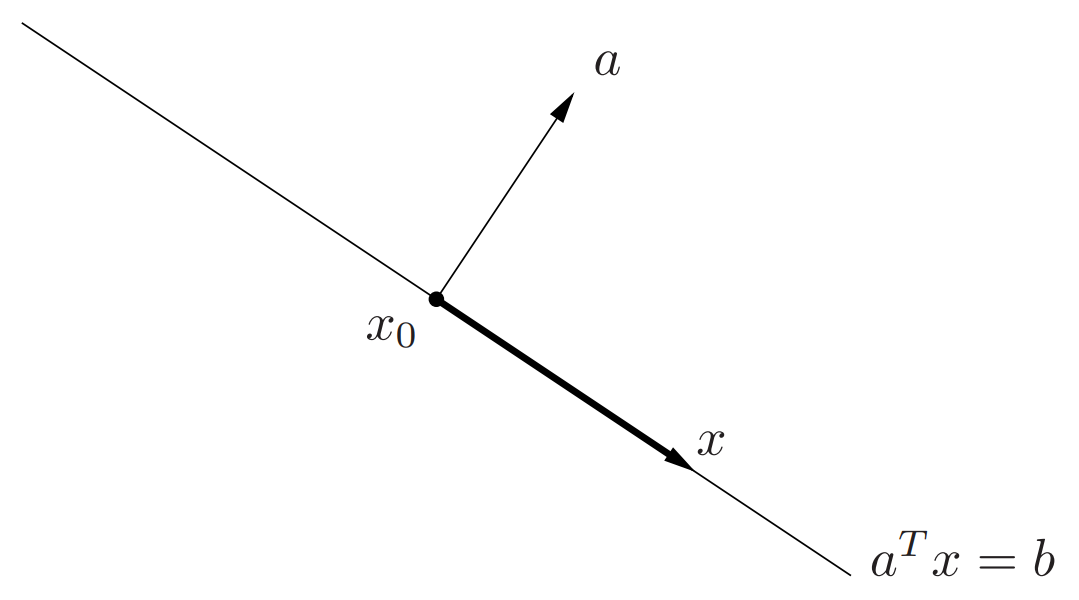
\includegraphics[scale=0.2]{hyperplane.png}
            \vspace{-5 pt}
            \caption{
                A hyperplane with normal vector $ \mathbf{a} \in
                \mathbb{R}^2 $. Note $ \mathbf{a}^\top(\mathbf{x} -
                \mathbf{x}_0) = 0 $\footnote{
                    Figure 2.6 from Boyd and Vandenberghe's
                    \textit{Convex Optimization}.                
                }.
            }
            \label{fig:hyperplane}
            \vspace{-5 pt}
        \end{figure}

        \item
        As seen in Figure \aref{fig:hyperplane}, for hyperplane
        $ L \triangleq \{\mathbf{x} \in \mathbb{R}^n :
        \mathbf{a}^\top\mathbf{x} = b \} $,
        $ \forall \mathbf{x}, \mathbf{y} \in L $,
        $ \mathbf{a}^\top(\mathbf{x} - \mathbf{y}) = 0 \Rightarrow \mathbf{a} $
        is orthogonal to vectors parallel to $ L $.
    \end{itemize}
\end{frame}
%
%\subsection{Primal formulation}
%
%\begin{frame}{Primal formulation}
%    \begin{itemize}
%        \item
%    \end{itemize}
%\end{frame}
%
%\subsection{Dual formulation}

% BibTeX slide for references. should use either acm or ieeetr style
\begin{frame}{References}
    \bibliographystyle{acm}
    % relative path may need to be updated depending on .tex file location
    \bibliography{../master_bib}
\end{frame}

\end{document}